\documentclass{report}  
\usepackage[utopia]{mathdesign} 
%\usepackage{amsmath,amsfonts,amsthm,amssymb,mathtools}

\input{preamble.tex}

\usepackage{amsmath,amsthm,mathtools}
\usepackage{titlesec}
\usepackage{microtype}
\definecolor{myblue}{RGB}{0,82,155}




%\usepackage[scr]{rsfso}

%\usepackage{libertine}
%\usepackage{mathpazo}
%\usepackage{palatino}
%usepackage{crimson}


\newcommand{\faketarget}{\oplus\!\!\!\!\odot}
\newcommand{\target}{%
  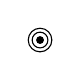
\begin{tikzpicture}[scale=0.5]
    \fill[black] (0,0) circle (0.1);
    \draw (0,0) circle (0.2);
    \draw (0,0) circle (0.3);
  \end{tikzpicture}%
}

\usepackage[clock]{ifsym}


\title{\Huge{Interface Personne Marchine}\\{IFT2905}\\{\textbf{Introduction}}}
\author{\huge{Franz Girardin}}
\date{\today}
\lstset{inputencoding=utf8/latin1}

            %%%%%%%%%%%%%%%%%  Sect.                          %%%%%%%%%%%%%%%%%%%%%%%%%%%%%%%%%%%%%%%%%%%%%%%%%%%%%%%%%
\usepackage{helvet}
\titleformat{\chapter}[display]
  {\normalfont\bfseries\color{myblue}}
  {\filleft%
    
\begin{tikzpicture}
    \node[
      outer sep=0pt,
      text width=1.5cm,
      minimum height=2cm,
      fill=myblue,
      font=\color{white}\fontsize{40}{50}\selectfont,
      align=center
      ] (num) {\thechapter};
    \node[
      rotate=90,
      anchor=south,
      font=\color{black}\Large\normalfont
      ] at ([xshift=-5pt]num.west) {\textls[180]{\textsc{Section}}};  
    \end{tikzpicture}%
  }
  {5pt}
  {\titlerule[2.0pt]\vskip3pt\titlerule\vskip4pt\large\normalfont}

\titleformat{\section}
  {\normalfont\scshape}{\thesection}{1em}{}



\titleformat{\section}
  {\normalfont\scshape}{\thesection}{1em}{}


% Customizing the spacing for the chapter titles
\titlespacing*{\chapter}{0pt}{0pt}{20pt}

%\usepackage[utopia]{mathdesign}
% Allow hfill in math environment
\newcommand{\specialcell}[1]{\ifmeasuring@#1\else\omit$\displaystyle#1$\ignorespaces\fi}

% Allow you to do the non implication (implication barred)
\newcommand{\notimplies}{%
  \mathrel{{\ooalign{\hidewidth$\not\phantom{=}$\hidewidth\cr$\implies$}}}}



\DeclareRobustCommand{\looongrightarrow}{%
  \DOTSB\relbar\joinrel\relbar\joinrel\relbar\joinrel\rightarrow
}

\begin{document}
%\maketitle

\pagebreak

\pagebreak
\begin{multicols*}{3}


    \footnotesize
    %\section*{Design of everyday things}

    \chapter{\textsc{Why Design fails \& Design of Everyday Things}}


    \paragraph{Mythe de l'erreur humaine} $\mathcal{H}$   
    Les \textit{échecs} d'un système $\mathbb{PM}$ sont souvent dus  
    au \textbf{design}. Pour $\downarrow$ erreur $\mathcal{H}$ : 
    \begin{itemize}
        \item[$\rhd$ ] Design qui tient compte des \textbf{limitations}
            et de la \textbf{fiabilité} des $\mathcal{H}$.   
    \end{itemize}

    \paragraph{Principes de design}
    \begin{itemize}
        \item[$\rhd$] Utilisabilité
        \item[$\rhd$] Expérience de l'Utilisateur ($\mathbb{UX}$)
        \item[$\rhd$] \textbf{Psychopathologie} : frustratiosn courantes  
         \item[$\blacktriangleright$] Permettent de 
             \textbf{critiquer}, \textbf{analyser} et \textbf{convervoir} interfaces.     

    \end{itemize}


    \paragraph{Causes d'échecs}
    \begin{itemize}
        \item[$\rhd$] Fonctionnalité 
            \begin{itemize}
                \item[$\blacktriangleright$] $\mathcal{U}$ ne connait pas fonctions de l'Obj.
                \item[$\blacktriangleright$] L'objet ne fait pas ce que  
                    $\mathcal{U}$ désire. 
            \end{itemize}
        \item[$\rhd$] Visibilité 
            \begin{itemize}
                \item[$\blacktriangleright$] $\mathcal{U}$ \textbf{voit} 
                    pas certaines infos l'Obj.   
                \item[$\blacktriangleright$] 
                    $\mathcal{U}$ ne sait pas quelle séquence de contrôle est nécessaire pour 
                    atteindre son but.  
                \item[$\rhd$] E.g. Lumières enfoncée pour passage piétons
            \end{itemize}
        \item[$\rhd$] Feedback 
            \begin{itemize}
                \item[$\blacktriangleright$] Comment $\mathcal{U}$ 
                    sait si les opérations ont réussi ?
                \item[$\blacktriangleright$] 
                    Comment $\mathcal{U}$ 
                    sait s'il y a une erreur en cours de route ?
            \end{itemize}
    \end{itemize}

    \paragraph{Buts du $\mathbb{UX}$ | }
    $\mathbb{MAUSSEE}$ : $\mathbb{M}$émorabilité, 
    $\mathbb{A}$pprentissage, $\mathbb{U}$tilité,
    $\mathbb{S}$écurité, $\mathbb{S}$atisfaction, 
    $\mathbb{E}$fficience, $\mathbb{E}$fficacité. 

    \paragraph{Définition de l'utilisabilité}
    Degré selon lequel un produit peut être utilisé par des 
    $\mathcal{U}$ \textit{identifiés}, pour atteindre des 
    \textbf{buts} \textit{définis} par 
    l\textbf{'efficacité}, l\textbf{'efficience} et 
    la \textbf{satisfaction}.   
    \begin{itemize}
        \item [$\rhd $] \textbf{ Efficacité} : atteindre le but \;  $\target$
        \item [$\rhd $] \textbf{ Efficience} : \textit{effort} 
            et ou \textit{temps} \textbf{minimal} \; \showclock{0}{45} 
        \item [$\rhd $] \textbf{ Satisfaction} :  
            évaluation subjective par $\mathcal{U}$
    \end{itemize}

    \begin{note}{}{}
        L'\textbf{utilisabilité} implique aussi la sécurité, l'apprentisage 
        et la \textit{mémorabilité}.   
    \end{note}

    \paragraph{Où les desginer se trompent}  
    \begin{itemize}
      \item [$\rhd $] Ne comprennet pas $\mathcal{U}$ et leurs limitations
      \item [$\rhd $] Ne prévoient pas différents \textbf{contextes d'utilisation}  
      \item [$\rhd $] Absence de \textbf{modèle détaillé} du fonct.        
      \item [$\rhd $] Absence de \textbf{feedback} par l'objet.        
    \end{itemize}

    \paragraph{Pourquoi le design est-il difficile}
    Les \textbf{interactions} sont complexes et difficile à définir. Par ailleurs, les tâches 
    sont complexes et \textit{implicites}. Il faut distribuer \textit{raisonnablement}
    les tâches à la machine et à l'$\mathcal{U}$ pour éviter que l'un ou l'autre 
    ne soit pas confronté à une complexité excessive. 

    \paragraph{Principe de découvrabilité}
    L'$\mathcal{U}$ doit savoir immédiatement à quoi l'objet sert, comment 
    l'utiliser et quelles sont les opérations possibles. 

    \begin{itemize}
      \item [$\rhd $]  \textbf{Affordance} ce que l'O permet de faire.  
            Un \textit{signifiant} est un élément qui permet de rendre 
            \textbf{l'affordance} visible.   

      \item [$\rhd $]  \textbf{Signifiants} indiquent que l'affordance 
        $\exists$ et ne doivent pas être \textbf{contradictoire}.   

      \item [$\rhd $]  \textbf{Anti-affordance} permettent de masquer 
        visibilité d'un aff. et contribue à la gestion d'erreur. 
        Il s'agit d'une affordance qui est \textit{délibérément supprimée}

      \item [$\rhd $]   \textbf{Correspondance} Permet de faire 
        l'association lors de l'utilisation 
        (direction volume, mode \texttt{on}/\texttt{off})
        \begin{itemize}
          \item [$\blacktriangleright$] Soit une série de lumières alignées et des interrupteurs un à côté 
            de l'autre, quel interrupteur alume quelle lumière. 
        \end{itemize}
        
        \item [$\rhd$ ] \textbf{Contraintes}  
          sont des restrictions physiques ou logiques de l'objet ou l'interface 
          qui contraignent l'$\mathcal{U}$à utiliser l'objet d'une certain façon. 
          P. ex., orientation d'une \textit{clé USB}.   

        \item [$\rhd$ ] \textbf{Feedback} permet d'indiquer à l'$\mathcal{U}$     
          l'effet de son action ou d'une interaction. 

        \item [$\rhd$ ] \textbf{\textcolor{red}{Modèle conceptuel}}
          est une explication très simplifiée 
          du fonctionnement d'un élément. 
          \begin{itemize}
            \item [$\blacktriangleright$ ] \textbf{Modèle fonctionnel} : on sait \textit{quoi} 
              faire sans savoir \textit{pourquoi} ça marche       
            \item [$\blacktriangleright$ ] \textbf{Modèle structurel} : on connait 
              les composants et leurs interactions
            \item[ $\rhd$] Exemple : \textit{Chinese mystery pot}  
          \end{itemize}
        
    \end{itemize} 




    \paragraph{Les deux fossés d'interaction}
    La conception doit permettre de résoudre \textbf{2} ensembles de questions 
    que l'$\mathcal{U}$ se pose lorsqu'il interagit :
    \begin{itemize}
      \item [$\blacktriangleright$ ] Comment ça marchee et 
        \textit{qu'est-ce que je peux faire avec l'objet ?}  
      \item [$\blacktriangleright$ ] Qu'est-ce qui s'est passé et 
        \textit{est-ce que c'est ce que je voulais faire ?}  
    \end{itemize}

    \paragraph{Les sept étape d'une actions}
    1. Définitir l'\textit{objectif}, 2. Former l'\textit{intention}    
    3. Spécifier la séquence d'actions, 4. Exécuter l'action
    5. Percevoir l'état du système 6. Interpréter l'état du système 
    7. Évaluer l'état du syst. \textit{par rapport aux intentions}.   


    \paragraph{Analyse de la cause originelle}
    Permet de déterminer si un \textit{objectif} est réelle 
    la fin souhaitée ou est simplement un sous-objectif 
    d'un but à atteindre. 

    \paragraph{Septs questions garantissant l'atteinte de l'O}
    Un \textit{bon design} implique qu'à tout moment, l'$\mathcal{U}$ 
    parvient à répondre aux \textbf{sept questions} suivantes.   

    1. Que puis-je faire, 2. Quelles sont les alternatives 
    3. Comment puis-je le faire, 4. Le fais-je bien ? 
    5. Qu'est-ce que ça veut dire 6. Que s'est-il passé ? 


  \dirtree{%
  .1 \textcolor{myb}{\textbf{Mythe de l'erreur humaine}}.
  .2 Importance du design dans la réduction des erreurs humaines.
  .1 \textcolor{myb}{\textbf{Principes de design}}.
  .2 Utilisabilité.
  .2 Expérience de l'Utilisateur (UX).
  .2 Psychopathologie.
  .1 \textcolor{myb}{\textbf{Causes d'échecs}}.
  .2 Fonctionnalité.
  .3 Connaissance des fonctions par l'utilisateur.
  .3 Adéquation des fonctions aux besoins de l'utilisateur.
  .2 Visibilité.
  .3 Visibilité des informations.
  .3 Clarté sur les séquences de contrôle nécessaires.
  .2 Feedback.
  .3 Indication de la réussite des opérations.
  .3 Signalement des erreurs.
  .1 \textcolor{myb}{\textbf{Buts du UX}}.
  .2 Mémorabilité, Apprentissage, Utilité, Sécurité, Satisfaction, Efficience, Efficacité.
  .1 \textcolor{myb}{\textbf{Définition de l'utilisabilité}}.
  .2 Efficacité.
  .2 Efficience.
  .2 Satisfaction.
  .1 \textcolor{myb}{\textbf{Où les designers se trompent}}.
  .2 Compréhension des utilisateurs et de leurs limitations.
  .2 Prévision des différents contextes d'utilisation.
  .2 Modélisation détaillée du fonctionnement.
  .2 Feedback de l'objet.
  .1 \textcolor{myb}{\textbf{Pourquoi le design est-il difficile}}.
  .2 Complexité des interactions et distribution des tâches.
  .1 \textcolor{myb}{\textbf{Principe de découvrabilité}}.
  .2 Affordance.
  .2 Signifiants.
  .2 Anti-affordance.
  .2 Correspondance.
  .2 Contraintes.
  .2 Feedback.
  .2 Modèle conceptuel (fonctionnel et structurel).
  .1 \textcolor{myb}{\textbf{Les deux fossés d'interaction}}.
  .2 Compréhension du fonctionnement et validation des actions.
  .1 \textcolor{myb}{\textbf{Les sept étapes d'une action}}.
  .2 Définition de l'objectif à l'évaluation des résultats.
  .1 \textcolor{myb}{\textbf{Analyse de la cause originelle}}.
  .2 Détermination des objectifs réels et sous-objectifs.
  .1 \textcolor{myb}{\textbf{Sept questions garantissant l'atteinte de l'objectif}}.
  .2 Questions clés pour un bon design.
  }


    \chapter{Design Centré sur $\mathcal{U}$}

    \paragraph{Risque du modèle en cascade}
    Il permet de s'assurer que les implémentation sont  
    \textit{conformes aux engiences}, mais ne garantit pas qu'elles sont 
    optimales pour $\mathcal{U}$. Par ailleurs, les 
    problèmes sont parfois identifiés plus tard et 
    revenir en arrière dans la modèle cascade peut être \textbf{couteux}
    \begin{itemize}
      \item [$\rhd$ ] Problèmes identifiés tard.  
      \item [$\rhd$ ]  Manque d'input et \textit{feedback} de l'$\mathbb{U}$  
      \item [$\rhd$ ] Problèmes $\rightarrow$ 
                        modif. exigences et conception.   
    \end{itemize}


    \paragraph{Design itératif}
    Étale le projet sur plusieurs petites itérations
    de \textit{conception}, \textit{prototypage} et 
    \textit{évaluation}.  


    \paragraph{Modèle en spirale}
    Il utilise le principe de design itératif et réduit graduellement 
    les risques à travers le \textit{itérations}. 
    Seules les itérations matures sont présentée à l'$\mathcal{U}$. 

    \paragraph{Design centré sur l'$\mathcal{U}$ }
    Marque un changement de paradigme où l'opinion 
    de l'$\mathcal{U}$ a précédence sur la \textit{technologie}  
    ou l'intuition du designer. On conçoit en fonction de 
    ce que les $\mathcal{U}$ \textit{doivent}, \textit{peuvent} 
    ou \textit{veulent} faire.   \\
      \noindent
      $\rhd$ \textbf{Prédesign} pour comprendre le problème  
      \\
      $\rhd$ \textbf{Premier design} pour explorer l'espace de design  
      \\
      $\rhd$ \textbf{Mi-design} Développe l'approche choisie  
      \\
      $\rhd$ \textbf{Design avancé} lorsqu'on intègre et déploie   
    L'évaluation par les $\mathcal{U}$ se fait de façon \textit{continue}; 
    ils accompagnent les développement à chaque itération:

    
    \paragraph{Design}
    Il faut \textbf{1.}  analyser les utilisateurs, les tâches 
    \textit{qu'ils cherchent à accomplir}; il faut comprendre le problème 
    et s'assurer que l'idée de solution est importante ou au moins 
    \textit{nécessaire} pour les $\mathcal{U}$. Il faut estimer le 
    niveau d'expertise des $\mathcal{U}$. Il faut aussi \textbf{2.}  
    suivre les principes de conceptions liés à l'\textit{utilisabilité}  
    Finalement, il faut \textbf{3.} assurer la prévention 
    et gestion des erreurs. 

    \paragraph{Implémentations brouillons}
    Elle peut être sur papier ou de style \textit{Wizard of Oz}  
    C'est \textit{rapide}, \textit{simple} et suffisamment 
    \textit{abstrait} pour se concentrer sur l'essentiel.   


    \paragraph{Évaluation}
    Permet de relier la \textit{progression de la conception} aux 
    \textit{besoin indentifiés} et aux contextes de l'utilisateur. 
    L'évaluation peut être effectué \textit{tôt} ou \textit{tard}, 
    selon le besoin. 


    \paragraph{Identifier les parties intéressées}
    Cela dépend de plusieurs questions :
    \dirtree {%
    .1 Parties intéressées.
    .2 qui l'utilisera?.
    .2 qui décidera de l'utiliser?.
    .2 qui va payer pour cela?
    .2 qui doit le faire (concevoir / construire)?.
    .2 qui doit en tirer profit?.
    .2 qui rendra votre vie misérable.
    }

    \chapter{Évaluation heuristique}

    \paragraph{Types d'erreurs}
    \mbox{}\vspace{0.4em}
  
    \noindent$\blacktriangleright$
    \textbf{Bévues} et \textbf{Lapsus} sonts causés par 
        \textit{manque reflexion}  

    \noindent  $\rhd$ \textbf{Bévues} $\looongrightarrow$ échec d'exécution.    

    \noindent  $\rhd$ \textbf{Lapsus} $\looongrightarrow$ faille de 
    mémoire lors de l'exec.  

    \noindent $\rhd$ \textbf{Méprise} est un échec de mémoire et ou planif. P. ex., 
        planifier procédures selon objectif, mais procédures utilsées 
        ne mènent pas à l'objectif (méprise sur le choix de procédure). 


    \dirtree{%
    .1 Type d'erreurs.
    .2 Erreur d'\textit{exécution}.  
    .3 Lapsus. 
    .4 Perte d'intention.
    .4 Omission due à l'interruption. 
    .4 Omission due à la satisfaction.
    .3 Bévues. 
    .4 De Capture.
    .4 De Description.
    .4 De Mode. 
    .2 Méprises.
    }

    \noindent $\rhd$ \textbf{Erreur de capture} Survient 
    lorsqu'un \textit{comportement fréquent} capture notre attention et 
    nos action. P. ex. vouloir taper \texttt{facial recognition} sur 
    Google et finir par naviguer sur facebook. 


    \noindent $\rhd$ \textbf{Erreur de description} Survient 
    lorsqu'une \textit{description} n'est pas suffisamment précise. 
    P. ex. confondre les logos \texttt{Reply} et \texttt{Replay All}.    


    \noindent $\rhd$ \textbf{Erreur de mode} Survient 
    lorsqu'on utilise un \textit{contrôle} dans un contexte 
    différent de celui qu'on souhaite. P. ex. utiliser 
    \texttt{j} ou \texttt{k} dans d'autres application que \texttt{Vim}.

    \paragraph{Stratégies pour prévenir les erreurs}
    \begin{itemize}
      \item [$\rhd$ ] \textbf{Bévues }  Éviter actions aux démarches similaires
      \item [$\rhd$ ] \textbf{Lapsus} Fonctions de \textit{forçage}   
      \item [$\blacktriangleright$ ]  Obliger retrait carte ATM 
        pour prendre \texttt{\$}  
      \item [$\rhd$ ] \textbf{Erreur de mode} Éliminer mode 
        ou $\uparrow$ \textit{visibilité} modes.   
    \end{itemize}

    \paragraph{Stratégies générales}
    \begin{itemize}
      \item [$\rhd$ ] Désactiver \textit{commandes illégales}  
      \item [$\rhd$ ] Rendre informations \textit{nécessaires} visibles  
      \item [$\rhd$ ] Préférer les listes déroulantes aux zones de texte 
      \item [$\rhd$ ] Utiliser les \textit{dialogue de confirmation}  
      \item [$\blacktriangleright$ ] Vous êtes sur le point de \texttt{rm -rf} !    
    \end{itemize}

    \paragraph{Contrôle par l'utilisateur et liberté}
    L'interface doit encourager l'exporation en rendant les choses visibles 
    et en assurant que les conséquences des erreurs ne soient pas sévères. 
    \[ \text{Exploration } \implies \uparrow \text{ Découvrabilité}\]. 
    

    \noindent $\rhd {}$ S'il y a \textbf{automatisation}, les changements doivent 
    aussi pouvoir être effectués manuellement. L'automatisation ne doit 
    pas \texttt{override} l'autonomie de $\mathcal{U}$. Les saisies
    \texttt{(input)} doivent être. Un $\mathcal{U}$ doit pouvoir 
    créer, modifier, lire, mettre à jour et supprimer toute donnée. 
    \textbf{modifiables}  
    
    \paragraph{Le droit d'annuler} implique que 
    L'$\mathcal{U}$ doit pouvoir décider; les opérations doivent être annuables, 
    et toutes boîtes de dialogue doit avoir un bouton d'annulation, pour ne pas 
    \textbf{piéger}  

    \section{Évaluation heuristique}
    \paragraph{Avantages} Peut être fait rapidement, sans 
    équipement, sans $\mathcal{U}$ et pour peu de \$. 



    \begin{figure}[H]
      \begin{center}
        \includegraphics[width=0.35\textwidth]{DixHeur.jpg}
      \end{center}
    \end{figure}

    \paragraph{Étapes d'une évaluation heuristique}
    \begin{itemize}
      \item [$\rhd $] \textbf{Mise en place} préparation du matériel 
        (scénarios, protoype, liste d'heuristiques)  
      \item [$\rhd$ ] \textbf{Évaluation} pas exploration de l'interface, application 
        des heuristiques génération de liste de problèmes
      \item [$\rhd $] \textbf{Agrégation}  retour et discusson entre experts.
    \end{itemize}   

    \begin{note}{}{}
      Il est important d'avoir \textbf{plusieurs évaluateurs} parce chacun d'eux peuvent 
        identifier \textit{différents problèmes}  
    \end{note}

    \paragraph{Évaluation}
    Il faut au moins \textbf{2 passages} par évaluation; le premier sert 
    à découvrir le flux de la plateforme et le second permet de 
    \textit{cibler} des éléments spécifiques.   

    \noindent $\rhd$ \textbf{Liste de problèmes} est produite par l'évaluateur; 
    il y mentionne \textit{l'heuristique qui est violée} et attribue 
    un \textbf{cote} de gravité.   

    \begin{figure}[H]
      \begin{center}
        \includegraphics[width=0.15\textwidth]{CotteGravite.png}
      \end{center}
    \end{figure}
    \vspace{-2em}

    \noindent $\rhd$ \textbf{Impact du problème}   

    \noindent $\rhd$ \textbf{Fréquence du problème}   


    \paragraph{Marqueurs de bon design}
    Les $\mathcal{U}$ n'attendent pas trop longtemps et on offre 
    du \textit{feedback} (visibilité); on utilise des mots, symboles
    et conventions
    qui \textit{match} avec le monde réel, p.ex \textit{trashbin}; 
    on \textit{ne force pas} l'utilisateur sur un chemin fixe; 
    on permet la révision, correction, modification, supression; 
    on \textit{rend les erreurs impossible} et valide les entrer; 
    on s'assure 
    que les tâche courantes se font de façon efficiente grâce aux 
    accélérateurs de calvier et souris, abréviations, double-clic,
    raccourcis 
    de menu et touches de fonction, etc.; on aide  
    l'$\mathcal{U}$ à reconnaître, diagnostiquer et récupérer 
    les erreurs; on offre de la documentation.


    \chapter{Design centré sur les tâches}

    \paragraph{Persona}
    Représentation symbolique de $l'\mathcal{U}$ décrivant 
    ses caractéristique et les \textit{tâches} qu'il doit 
    accomplir. 

     \paragraph{Parties intéressées \textit{Stakeholders}  }
     Réfère à toute personne ayant une 
     \textbf{raison} de se soucier à l'interface.   
     \begin{itemize}
       \item [$\rhd$ ] Souvent nombreux 
         \begin{itemize}
           \item [$\blacktriangleright $] Les $\mathcal{U}$ 
           \item [$\blacktriangleright $] Les \texttt{dev.}  
           \item [$\blacktriangleright $] Les constructeurs 
           \item [$\blacktriangleright $] Les sponsors 
         \end{itemize}
       \item [$\rhd$ ] Intérêts parfois en conflits
         \begin{itemize}
           \item [$\blacktriangleright $] Ces efficience, utilité 
           \item [$\blacktriangleright $] Facilité de dev. 
           \item [$\blacktriangleright $] Facilité de construction 
           \item [$\blacktriangleright $] Coût de financement 
         \end{itemize}
     \end{itemize}
     \noindent
     \section{Workflow du design centré sur les tâches}
     \texttt{
       Identification $\looongrightarrow$ 
       Exigences $\looongrightarrow$ 
       Design Conceptuel $\looongrightarrow$ 
       Parcour cognitif
     }  

     \paragraph{Identification}
     Identifier l'$\mathcal{U}$; analyser des \textit{exemples de
     tâche} 

     \paragraph{Exigences}
     Décider quelles tâches le design soutiendra.    
    \begin{note}{}{}
      Il \textit{faut} décrire les tâches à l'aide 
      \textbf{d'exemple de tâches imaginées}  pour pavenir 
      à déterminer les exigences. Les tâches peuvent être 
      décrites par leur fréquence et leur importance. 
    \end{note}

    \textbf{En pratique}, pour identifier les tâches, on peut 
    contacter les potentiels $\mathcal{U}$ et discuter 
    avec eux du fonctionnement du système pour avoir  
    leur feedback. Il faut demander à l'$\mathcal{U}$
    de réviser les exemples de tâches : 
    \begin{itemize}
      \item [$\rhd$ ] Omissions 
      \item [$\rhd$ ] Corrections
      \item [$\rhd$ ] Clarifications
      \item [$\rhd$ ] Suggestions
    \end{itemize}


    \paragraph{Clarification de la distinction tâche-activité}
    Dans le 
    \textit{design centré sur les tâches}, 
    le mot \textit{tâche}  
    a une signification plus proche du mot 
    \textbf{activité}, puisque le design comprends 
    prend en compte une grande quantité de tâche et leur 
    contexte d'exécution. 


    \paragraph{Bon exemples de tâches} 
    Ils sont décrivent \textbf{quoi} sans extrapoler 
    \textbf{comment}; il sont 
    \textit{spécifiques}; ils sont \textit{exhaustif} et décrivent 
    le travail de l'$\mathcal{U}$ dans son ensemble ainsi que 
    la transmission globale de l'information. 
    Dans l'ensemble, 
    ils reflètent les intérêt des vrais $\mathcal{U}$. 

     \paragraph{Design conceptuel}
      Décrire la base d'interaction et de représentation 
      (modèle mental). On utilise un \textbf{scénario} :

      \[ \texttt{tâche + design } = \texttt{scénario}    \]
    Le scénario montre comment une tâche est gérée par le 
    design. 

    \begin{align*}
      &\textbf{Tâche } \colon 
          \texttt{Elle choisit une recette dans la liste} \\
      &\textbf{Scénario} \colon     
          \texttt{Elle fait \textcolor{myg}{défiler la liste} 
        d'images} \\ 
      &\texttt{et \textcolor{myg}{tape sur}\dots  }  
    \end{align*}        


    \paragraph{Parcours cognitf}
    Parcourir le tâches \textit{pas à pas} en utilisant le 
    design et \textbf{évaluer}.   


    \paragraph{Avantages de design centré sur les tâches}
    \begin{itemize}
      \item [$\blacktriangleright$ ] Permet de baser le design 
        sur $\mathcal{U}$ et \textit{tâches réelles}  
      \item [$\blacktriangleright$ ] Permet d'identifier les 
        exigences lors de la \textit{phase pré-design} 
        (avant même design conceptuel). 
    \end{itemize}

    \chapter{Les exigenbces du design}


    \paragraph{Types d'exigences}
    \begin{itemize}
      \item [$\rhd$ ] \textbf{Fonctionnelle} : ce que le produit 
        doit faire
       \item [$\rhd$ ] \textbf{De données} : caractéristiques des 
         données requises 
      \item [$\rhd$ ] \textbf{D'environnement}  :  Contexte
        physique 
        et non physique nécessaires au fonctionnement. 
      \item [$\rhd$ ] \textbf{Propres à l'$\mathcal{U}$}   
        \begin{itemize}
          \item [$\blacktriangleright$ ] P. ex. une 
            \textit{mère célibataire}  
        \end{itemize}

    \end{itemize}


    




     


    \end{multicols*}

\end{document}
